\documentclass{sig-alternate}
\usepackage[backend=bibtex,style=numeric-comp]{biblatex}
\usepackage{tikz}

\newcommand{\code}[1]{\texttt{#1}}

\author{
\alignauthor{}
Dan Stelljes\\
  \affaddr{Division of Science and Mathematics}\\
  \affaddr{University of Minnesota, Morris}\\
  \affaddr{Morris, Minnesota, USA 56267}\\
  \email{stell124@morris.umn.edu}
}
\conferenceinfo{UMM CSci Senior Seminar Conference, December 2016}{Morris, MN}
\title{Composable Concurrency Models}

\bibliography{references}

\AtEveryBibitem{\clearfield{doi}}
\AtEveryBibitem{\clearfield{note}}

\begin{document}

\maketitle

\begin{abstract}

The need to manage concurrent operations in applications has led to the development of a variety of concurrency models. Modern programming languages generally provide several concurrency models to serve different requirements, and programmers benefit from being able to use them in tandem. We discuss challenges surrounding concurrency control and examine situations in which conflicts between models can occur. Additionally, we describe attempts to implement concurrency models on top of lower-level concurrency abstractions.

\end{abstract}

\keywords{concurrency, parallelism, concurrency abstraction}

\section{Introduction}

Most interactive computer programs depend on concurrency, the ability to perform different tasks at the same time. A web browser, for instance, might at any point be rendering documents in multiple tabs, transferring files, and handling user interaction. On a lower level, the operating system might be running several other applications, juggling background processes, and responding to events~\cite{Swalens2014}. If every long-running process blocked other processes from proceeding, the system would be effectively unusable.

Concurrency models enable programmers to reason about and describe interactions between concurrent processes. The web browser is a good example of several different models: The user interface layer might rely on an event loop, the rendering process might operate in shared memory, and suggestions from browsing history or a search engine might require parallel collection operations or map-reduce to achieve acceptable performance~\cite{Marr2012}.

Given that an application is likely to make use of more than one concurrency model, programmers would prefer that different models could be combined. Composability is also desirable from an engineering standpoint---a virtual machine for one or more high-level languages should be able to support a variety of models without sacrificing semantics or performance. However, different concurrency models are not necessarily composable and unexpected issues may arise when they interact. Recent work has attempted to identify unifying concurrency abstractions that would guarantee composability of different models and also provide underlying virtual machine support~\cite{Marr2009, Marr2012, Swalens2014, Ziv2015}.

\section{Background}

Modern operating systems are expected to run many processes concurrently, and processes themselves are often composed of multiple concurrent threads of execution. A processor can only execute one thread at a time, so multitasking is accomplished by rapidly switching between threads~\cite{Liu1973}. Although concurrent threads may appear to be executed simultaneously, truly parallel execution can only take place across multiple processors.

Concurrency models can abstract over implementation details, allowing programmers to reason in terms of asynchronous tasks and independent components instead of low-level thread management. In addition to making a program more understandable, higher-level models afford a degree of flexibility: Concurrent operations could be executed in an event loop on one thread, executed in multiple threads on the same processor, or executed in parallel.

\subsection{Concurrency}

For operations to be executed concurrently, they must be able to be executed out of order or in partial order. Lamport, in his foundational work on distributed systems, formalized this by defining a ``happens before'' relation (denoted by ``$\rightarrow$'') on a set of operations: If $A$ and $B$ are operations in the same process and $A$ occurs before $B$, or if $A$ is the sending of a message by one process and $B$ is the receipt of the same message by another process, then $A \rightarrow B$. Two operations $A$ and $B$ are said to be concurrent if $A \nrightarrow B$ and $B \nrightarrow A$~\cite{Lamport1978}.

While the ``happens before'' relation can be used to determine whether operations can be executed concurrently, it does not guarantee the correctness of the results. In a non-concurrent (entirely sequential) program, it would be sufficient to show that the program is correct after the execution of each operation and therefore correct upon termination. In other words, the program could be proved to be correct by proving that its history (that is, the sequence in which its operations are performed) yields a correct result. Consistency models guarantee the correctness of a program by defining a set of all allowed histories~\cite{Ziv2015}. If an execution of a program follows an allowed history, the execution is consistent. If not, the execution is inconsistent. If every possible execution of the program follows an allowed history, the program conforms to the consistency model.

\begin{figure}[h]
  \centering
  \begin{tikzpicture}
    \draw [|-|] (0,0) node[left=3pt] {$ x $} -- (6,0);

    \draw [<-] (0.5,0.25) -- (0.5,0.75) node[above=3pt] {$ 1 $};
    \draw [->] (1,0.25) -- (1,0.75) node[above=3pt] {$ 1 $};

    \draw [<-] (2,0.25) -- (2,0.75) node[above=3pt] {$ 2 $};
    \draw [->] (2.75,0.25) -- (2.75,0.75) node[above=3pt] {$ 2 $};
    \draw [->] (3.25,0.25) -- (3.25,0.75) node[above=3pt] {$ 2 $};

    \draw [<-] (3.75,0.25) -- (3.75,0.75) node[above=3pt] {$ 3 $};

    \draw [<-] (4.5,0.25) -- (4.5,0.75) node[above=3pt] {$ 4 $};
    \draw [->] (5.5,0.25) -- (5.5,0.75) node[above=3pt] {$ 4 $};
  \end{tikzpicture}
  \caption{A single thread writes to and reads from a single variable.}
\label{figure:single}
\end{figure}

Figure~\ref{figure:single} illustrates a simple program in which a single thread reads and writes numbers from a variable $x$. (Write operations are denoted by an arrow pointing toward the line and read operations by an arrow pointing away.) The program satisfies an intuitive model of how variables should behave---each time $x$ is read, the value is equal to the value of the most recent write.

\begin{figure}[h]
  \centering
  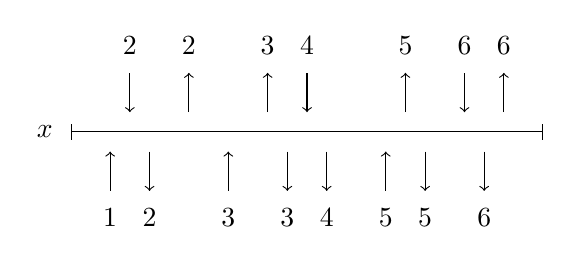
\begin{tikzpicture}
    \draw [|-|] (0,0) node[left=3pt] {$ x $} -- (6,0);

    \draw [<-] (0.5,-0.25) -- (0.5,-0.75) node[below=3pt] {$ 1 $};

    \draw [<-] (0.75,0.25) -- (0.75,0.75) node[above=3pt] {$ 2 $};
    \draw [->] (1,-0.25) -- (1,-0.75) node[below=3pt] {$ 2 $};
    \draw [->] (1.5,0.25) -- (1.5,0.75) node[above=3pt] {$ 2 $};

    \draw [<-] (2,-0.25) -- (2,-0.75) node[below=3pt] {$ 3 $};
    \draw [->] (2.5,0.25) -- (2.5,0.75) node[above=3pt] {$ 3 $};
    \draw [->] (2.75,-0.25) -- (2.75,-0.75) node[below=3pt] {$ 3 $};

    \draw [<-] (3,0.25) -- (3,0.75) node[above=3pt] {$ 4 $};
    \draw [->] (3.25,-0.25) -- (3.25,-0.75) node[below=3pt] {$ 4 $};

    \draw [<-] (4,-0.25) -- (4,-0.75) node[below=3pt] {$ 5 $};
    \draw [->] (4.25,0.25) -- (4.25,0.75) node[above=3pt] {$ 5 $};
    \draw [->] (4.5,-0.25) -- (4.5,-0.75) node[below=3pt] {$ 5 $};

    \draw [<-] (5,0.25) -- (5,0.75) node[above=3pt] {$ 6 $};
    \draw [->] (5.25,-0.25) -- (5.25,-0.75) node[below=3pt] {$ 6 $};
    \draw [->] (5.5,0.25) -- (5.5,0.75) node[above=3pt] {$ 6 $};
  \end{tikzpicture}
  \caption{Two threads concurrently write to and read from a single variable.}
\label{figure:multiple}
\end{figure}

In a concurrent program, the history of operations may not be the same for every execution. As a result, assumptions about correctness that are true for a sequential program may be violated in a concurrent program. This is illustrated in Figure~\ref{figure:multiple}, in which two threads concurrently write from and read to a variable $x$ concurrently. Because the operations of the threads are interleaved, a read operation on $x$ may not yield a value that matches the value of that thread's most recent write. The value may even be inconsistent between consecutive reads. (Errors that arise due to unintentional dependency on execution order are referred to as race conditions.) From the perspective of a single thread, the program appears to be incorrect because it violates the same intuitive model of how variables should behave.

\subsection{Linearizability}

The examples above assume that all operations complete instantaneously. In real systems, though, operations take time. Even writing to a location in cache memory, an operation measured in nanoseconds, is not truly instantaneous. That an operation may be completed at a time significantly later than the time at which it was invoked introduces uncertainty into a history of operations---the sequence of execution may be influenced by the time it takes for messages to travel.

\begin{figure}[h]
  \centering
  \begin{tikzpicture}
    \draw [|-|] (0,0) node[left=3pt] {$ x $} -- (6,0);

    \draw (0.75,0.25) -- (0.5,0.75) node [above left] {$ 1 $};
    \draw (0.75,0.25) -- (1,0.75);

    \draw (3.75,-0.25) -- (2,-0.75);
    \draw (3.75,-0.25) -- (5.5,-0.75) node [below right] {$ 2 $};

    \draw (3.25,0.25) -- (3,0.75) node [above left] {$ 2 $};
    \draw (3.25,0.25) -- (3.5,0.75);
  \end{tikzpicture}
  \caption{Two threads concurrently (and noninstantaneously) write to and read from a single variable.}
\label{figure:time}
\end{figure}

Consider a third example (Figure~\ref{figure:time}) in which two threads interact with a variable $x$ noninstantanously. (Invocation is denoted by the leftmost point of an event and completion by the rightmost point. The point closest to the line indicates the instant at which the operation takes effect.) The lower thread invokes a read while the value of $x$ is set to $1$. The upper thread invokes and completes a write between the time that the read is invoked and the value is actually read. The read operation then returns $2$ even though $x$ was equal to $1$ at the time it was invoked.

While travel time may introduce ambiguity, there are still some restrictions on possible sequences of events. Specifically, an operation cannot take effect before its invocation, nor can it take effect after its completion. Therefore, assuming that all threads share some single global state and that operations on that state take place atomically, each operation will appear to take effect atomically at some point after it is invoked and before it is completed.

This consistency model is referred to as linearizability (also referred to as atomicity or indivisibility), and it guarantees that the completion of an operation on a single object will appear to the rest of the system to be instantaneous~\cite{Herlihy1990}. In other words, even though linearizable operations are executed concurrently and take time, they appear to happen in a simple linear order.

A useful consequence of linearizability is that the results of an operation must be visible as soon as the operation is complete. This can prevent issues such as stale reads (in which a read operation returns a value different from the most recently written value) and non-monotonic reads (in which a later read operation returns an older value than an earlier read operation).

\subsection{Serializability}

A history of operations is said to be serializable if it is equivalent to a serial (i.e., non-interleaved) ordering of its operations~\cite{Herlihy1990}. Serializability is like linearizability in that it demands some linear order of execution. However, serializability describes multiple operations over multiple objects instead of single operations on single objects, and it does not impose any wall-clock time constraints on the history. This means that operations may occur in any order as long as some serial history exists.

Serializability alone is a fairly weak consistency model. Because it does not place bounds on time or order, events may happen out of sequence. However, serializability does guarantee isolation~\cite{Haerder1983}. In order for histories to be serializable, they must not overlap and cannot interfere with each other.

Together, linearizability and serializability guarantee strict serializability, in which a history is equivalent to a serial execution order and that order corresponds to the execution order in real time. Linearizability, then, can actually be described as strict serializability restricted to single operations on single objects~\cite{Herlihy1990}.

\section{Common concurrency models}

Modern programming languages generally provide several different concurrency models, each with their own terminology and specific implementation details. It would be impractical to discuss them all, but the most commonly used models can be adequately described by generalization~\cite{Swalens2014}.

\subsection{Atomic variables}

Atomic variables can only be read and mutated by operations that guarantee atomicity. For example, an atomic operation \emph{compare-and-swap} compares the current value of a variable to a given value and only performs a write if the values match~\cite{Swalens2014}. \emph{compare-and-swap} ensures that a new value cannot be written based on outdated information. Suppose that a thread $A$ reads a variable $v$ and begins computing a new value. At the same time, another thread $B$ modifies $v$. When $A$ tries to set the value of $v$ via \emph{compare-and-swap}, the write will fail. As a result, all writes on $v$ are guaranteed to be atomic.

Atomic operations like \emph{compare-and-swap} (and, similarly, \emph{fetch-and-add} and \emph{test-and-set}) are often implemented in hardware and guarantee linearizability at the lowest level possible. As such, atomic variables often serve as the basis for higher-level concurrency control mechanisms such as semaphores and locks, which in turn support the implementation of concurrent data structures. (Linearizability is a composable guarantee~\cite{Herlihy1990}; an operation made up of smaller linearizable operations is itself linearizable.)

A counting semaphore is an atomic variable that serves as a record of how many units of a shared resource are available. By taking advantage of atomic operations, the semaphore can be safely updated and will reliably determine whether a shared resource can be used. A single thread can then test if a resource is available and acquire it before proceeding, thereby preventing race conditions~\cite{Swalens2014}. A lock (also referred to as a mutex) guarantees mutual exclusion, which requires that two threads cannot operate on a shared object at the same time. Locks are commonly implemented by a binary semaphore (that is, a semaphore that simply indicates whether a single resource is available).

Higher-level languages (such as Clojure~\cite{Swalens2014}) often provide atomic references that can be read by an atomic dereferencing operation and written by an atomic swap operation. Such operations may provide convenience features such as automatic retries. In practice, atomics are used to share independent objects that do not demand coordinated updates~\cite{Swalens2014}.

\subsection{Software transactional memory}

Software transactional memory (STM) allows multiple concurrent operations to transactionally write to a shared location in memory. STM is an example of optimistic concurrency control: Each operation writes to the shared memory with no regard to the activity of other threads. After the entire transaction is completed, the transaction manager verifies that other threads have not also made changes to the shared memory. If there are conflicting changes, the transaction is aborted and re-executed until it eventually succeeds~\cite{Shavit1995}.

Conceptually, STM simplifies concurrency because it allows transactions to be thought of as a single-threaded operation. A thread cannot observe changes made to other threads while a transaction is in progress, nor can other threads observe modifications by that thread until the transaction is completed. Only when a transaction completes successfully will changes will become visible to other threads.

Harris and Fraser proposed the use of critical regions to represent transactions~\cite{Harris2014}.

\subsection{Communicating threads}

Instead of sharing memory, some concurrency models restrict operations to private memory. Threads communicate strictly by message passing, which avoids race conditions. Communicating sequential processes (CSP), one of the oldest communicating thread models, describes systems in terms of independent processes that communicate through predefined channels~\cite{Hoare1978}.

Other models, most notably the actor model, rely on asynchronous message passing to specific entities~\cite{Agha1986}. Actors can only communicate via asynchronous message passing. Upon receiving a message, an actor can choose to send messages to other actors, create new actors, and determine the behavior used for the next received message.

\subsection{Proxies}

Proxies are placeholders for values that are the result of some concurrently executed operation. Futures and promises are the two main types of proxy, though the terms are frequently used interchangeably (along with ``delayed'' and ``deferred''). Specifically, futures are resolved to the result of the completed operation. The result is then accessed implicitly; any use of the future will return its value. Promises can be created independently and require the result to be accessed explicitly.

\section{Correctness criteria}

\subsection{Safety}

Definition of safety as a guarantee of partial correctness (``nothing bad will happen'').

\subsection{Liveness}

Definition of liveness as a guarantee of progress and eventual termination (``something good will eventually happen'').

\section{Proposed abstractions}

More sources here would be good---Marr and D'Hondt~\cite{Marr2012} provide the only solid abstraction.

\subsection{Asynchronous events}

Ziarek et al.~\cite{Ziarek2011} introduce asynchronous events as a possible abstraction. Their examples are heavily tied to Concurrent ML and might be difficult to integrate.

\subsection{Ownership-based meta-object protocol}

Marr and D'Hondt~\cite{Marr2012} proposed an ownership-based meta-object protocol with the goal of providing VM support. They also demonstrate implementation of actors, STM, agents, and CSP.

\section{Conclusion}

In more words: There's a lot of work on the correctness of concurrent operations. With some care, concurrency models can be composed. There's some work on deeper abstractions, but it's definitely ongoing and more is likely to follow soon.

\section*{Acknowledgments}

Thanks to Elena Machkasova and K.~K. Lamberty for their patience and feedback.

\printbibliography{}

\end{document}
